\documentclass[tikz]{standalone}
\usepackage{pgfplots}
\pgfplotsset{compat=1.15}
\usepackage{mathrsfs}
\usetikzlibrary{arrows,calc}
\usepackage{tkz-euclide}
\pagestyle{empty}
\usepackage{fp}

\definecolor{AngleClr}{rgb}{0,0.39215686274509803,0}
\definecolor{ShapeClr}{rgb}{0.6,0.2,0}

\definecolor{BlueClr}{RGB}{5,81,163}

\begin{document}

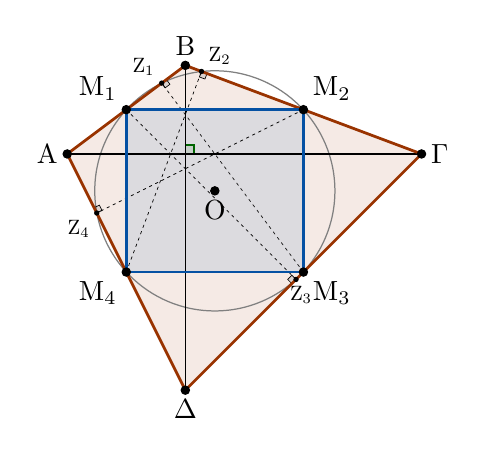
\begin{tikzpicture}[scale=.75]
\tkzSetUpLine[line width=1pt,color=black]
\tkzSetUpPoint[fill=black]

\tkzDefPoints{0/0/A,6/0/C,2/1.5/B,2/-4/D}

% Find the intersection of the diagonals.
\tkzInterLL(B,D)(A,C) \tkzGetPoint{I}

% Find the four midpoints.
\tkzDefMidPoint(A,B) \tkzGetPoint{M1}
\tkzDefMidPoint(B,C) \tkzGetPoint{M2}
\tkzDefMidPoint(C,D) \tkzGetPoint{M3}
\tkzDefMidPoint(D,A) \tkzGetPoint{M4}

% Find maltitude points.
\tkzDefPointsBy[projection=onto A--B](M3){Z1}
\tkzDefPointsBy[projection=onto B--C](M4){Z2}
\tkzDefPointsBy[projection=onto C--D](M1){Z3}
\tkzDefPointsBy[projection=onto D--A](M2){Z4}


\tkzFillPolygon[fill=ShapeClr,fill opacity=0.1,inner sep=1cm](A,B,C,D)
\tkzFillPolygon[fill=BlueClr,fill opacity=0.1,inner sep=1cm](M1,M2,M3,M4)

\tkzMarkRightAngle[line width=0.5pt, size=.15,color=AngleClr,fill=AngleClr,fill opacity=0.1](B,I,C)

% Find circle center.
\tkzDefMidPoint(M1,M3) \tkzGetPoint{O}
\tkzDrawCircle[line width=0.45pt](O,M1)

% Draw diagonals.
\tkzDrawSegment[line width=0.5pt,color=black](A,C)
\tkzDrawSegment[line width=0.5pt,color=black](B,D)

\tkzMarkRightAngles[line width=0.25pt, size=.1,color=black,fill=black,fill opacity=0.1](M1,Z3,D M2,Z4,A M3,Z1,B M4,Z2,C)

% Draw maltitudes.
\tkzDrawSegments[line width=0.25pt,color=black,dashed,dash pattern=on 1pt off 1.45pt](M1,Z3 M2,Z4 M3,Z1 M4,Z2)

\tkzDrawPolygon[color=ShapeClr](A,B,C,D)
\tkzDrawPolygon[color=BlueClr](M1,M2,M3,M4)
\tkzDrawPoints[size=3](A,B,C,D,M1,M2,M3,M4,O)
\tkzDrawPoints[size=1.5](Z1,Z2,Z3,Z4)

\tkzLabelPoint[left](A){$\rm A$}
\tkzLabelPoint[above](B){$\rm B$}
\tkzLabelPoint[right](C){$\rm \Gamma$}
\tkzLabelPoint[below](D){$\rm \Delta$}

\tkzLabelPoint[below](O){$\rm O$}

\tkzLabelPoint[above left](M1){$\rm M_1$}
\tkzLabelPoint[above right](M2){$\rm M_2$}
\tkzLabelPoint[below right](M3){$\rm M_3$}
\tkzLabelPoint[below left](M4){$\rm M_4$}

\tkzLabelPoint[scale=0.75,above left](Z1){$\rm Z_1$}
\tkzLabelPoint[scale=0.75,above right](Z2){$\rm Z_2$}
\tkzLabelPoint[scale=0.75,xshift=0.085cm,below](Z3){$\rm Z_3$}
\tkzLabelPoint[scale=0.75,below left](Z4){$\rm Z_4$}

\end{tikzpicture}

\end{document}
